% !TeX spellcheck = es_ES
\documentclass[arial,a4paper,print]{article}

\usepackage{helvet}
\usepackage{float}
\usepackage{graphicx}
\usepackage{subcaption}
\usepackage[labelfont=sc, font={footnotesize, singlespacing}]{caption}
\usepackage[margin=2cm]{geometry}  

\renewcommand{\familydefault}{\sfdefault}

\usepackage[spanish]{babel}
%opening
\title{Castellano: Selectividad 2022}
\author{tomiock}

\begin{document}
	
	\maketitle
	
Estos apuntes sobre lengua castellano los voy a hacer a partir de las orientaciones sobre el examen que te da la Generalitat (te dicen lo que sale básicamente). En vez de centrarme tanto en los contenidos y la resolución de los ejercicios, voy a hacer lo que llamo el 'metaestudio' es decir saber las cosas que va a salir y intentar planear que responder y que no. También sobretodo fijarme en los exámenes de anteriores años. 

\subsection{Opciones de la Prueba}
Antes de empezar hay que hablar de la opciones que te dan en este examen, que hay dos:
\begin{itemize}
\item Opción A:\\
Esta opción está más orientada a la literatura, el texto del cual tienes que hacer la compresión lectora suele ser una narración. 
\item Opción B:\\
Esta opción está más orientada a las tipologías textuales (expresión escrita) y el texto de la comprensión lectora suele ser un articulo de prensa \\
Yo voy a escoger esta opción siempre, ya que me parece más fácil resumir un texto a partir de sus argumentos que resumir una narración. También pienso hacer esto porque me es más fácil escribir un texto argumentativo con mis conocimientos generales, en vez de expresar una opinión o hacer un resumen de una de las lecturas obligatorias 
\end{itemize}
Hay que notar que la parte 3 (Reflexión Lingüística) no forma parte de estas dos opciones y es común. 
También he de decir que también las otras preguntas que forman parte de estas opciones (e.g. vocabulario o recursos literarios) se ven afectadas al escoger y se han de pensar en ellas a la hora de hacerlo. 

\section{Compresión Lectora}
\subsection{Resumen texto}
Lo más común es que pidan un \underline{resumen} del texto, sin embargo, también te puedes encontrar con una \underline{formulación del tema} o una \underline{asignación de títulos} a los párrafos. Cuanta un punto, así que es muy importante. Hay que pensar que el máximo son tan solo 40 palabras, lo mejor que se puede hacer es juntar frases importantes o 'key points' del texto. 

\subsection{Vocabulario}
Está pregunta depende más de suerte o de la cantidad de libros que te has leído en tu vida, más que de otra cosa. Aunque hay que ser inteligente y mirar bien al contexto en el cual se encuentran las palabras del texto para saber más o menos lo que significar. También es muy importante usar el descarte para acabar con una respuesta que al menos tenga pinta de estar bien. La última cosa que quiero decir sobre esta pregunta es que penalizan los errores así que a veces conviene no responder a un conjunto de palabras en particular si se da el caso. 

\pagebreak

\subsection{Compresión del texto}
En esta pregunta pueden preguntarte por tres cosas:
\begin{itemize}
\item Referentes/Antecedentes: En realidad te pueden preguntar dos cosas distintas en esta pregunta.  Un antecedente es el sustantivo/SN al que hace referencia un pronombre relativo o determinante relativo. Aquí tenéis una de esas preguntas como ejemplo:
\begin{figure}[H]
	\centering
	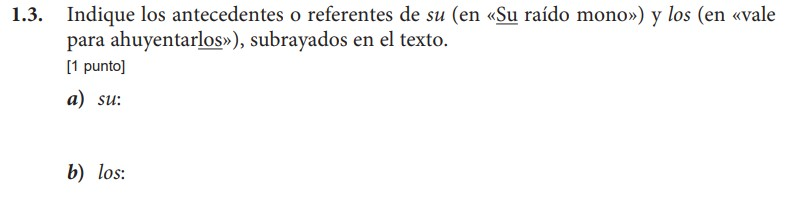
\includegraphics[width=0.8\linewidth]{figures/antecedente}
	\caption{Ejemplo de ejercicio de antecedentes. La respuesta \textbf{a)} es \underline{el casero} y la del \textbf{b)} es \underline{los mosquitos}.}
	\label{fig:antecedente}
\end{figure}

Para identificar un antecedente simplemente se puede hacer una sustitución o pregunta. Es algo bastante lógico en teoría. 

A veces no pregunta por un antecedente, sino por un referente\footnote{Es tricky porque un antecedente es un referente, pero no todos los referentes son antecedentes. (referente $\equiv$ palabras que se refiere a otra)}, en este caso pues es como más general, pero igualmente no debería de dar problema, aquí hay un ejemplo:
\begin{figure}[H]
	\centering
	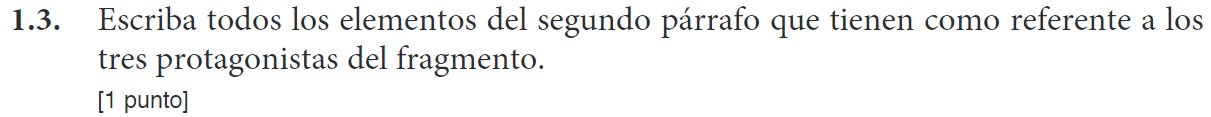
\includegraphics[width=0.8\linewidth]{figures/referente}
	\caption{Ejemplo de ejercicio de referente.}
	\label{fig:referente}
\end{figure}

\item Identificación de figuras retóricas: Esta es muy fácil, aquí tenéis una lista de las figuras que han salido a lo largo de los años: 
\begin{itemize}
	\item Metáfora: Identificación de dos objetos, real e imagen, en una misma frase. (no sé que quiere decir esta definición, perdón). Pero bueno, ya sabemos lo que es una metáfora, así que vamos a hablar de otros recursos literarios más complicados.
	\item Pleonasmo: Empleo de palabras superfluos o \underline{redundantes}: '\textit{enciende el cigarro apagado}'
	\item Paradoja:  Unión de dos términos en apariencia contradictorios: '\textit{a la vez quieto y en marcha}'
	\item Epanadiplosis: \underline{Repetición} de una palabra al principio y final de un verso u oración: '\textit{palabras de amor, palabras}' 
	\item Ironía: Afirmación de una idea, mediante la expresión contraria. 
\end{itemize}

Hasta aquí, las que han salido recientemente, ahora una lista de las que pueden salir:
\begin{itemize}
	\item Sinestesia: Cruce de dos imágenes sensoriales que proceden de sentidos distintos. 
	\item Metonimia: Designación de un objeto con el nombre de otro con el que guarda una relación. 
	\item Litote: Negación de aquello que se quiere afirmar. 
	\item Comparación/Símil: Relación, mediante un enlace, de un objeto real y un objeto imagen. 
	\item Anadiplosis: Repetición del último elemento de un grupo de palabras al principio del grupo siguiente.
	\item Anáfora: Repetición de una o más palabras a principio de los versos o enunciados sucesivos.
	\item Antítesis: Contraposición
\end{itemize}
En esta pregunta, pienso que conviene agrupar las figuras según su parecido (e.g. anadiplosis/epanadiplosis), porque cuando se ponen las opciones normalmente las figuras no tienen nada que ver entre si. También es común que pongan una figura que no sale en el currículum (hay muchísimas que no se estudian en realidad), para despistar, no la escojas. 

Para una lista exhaustiva y oficial de las que pueden salir referirse a  

\item Explicación del significado de una expresión: Esta tipo de pregunta, no tienen mucho misterio, es compresión lectora pura y dura. 
\end{itemize}

\subsection{Lecturas Obligatorias}
Hay tres preguntas y solo se deberá de contestar dos de ellas. Normalmente son muy fáciles (si te has leído la novela). Por ejemplo, en el último examen una de ellas era sobre el medio de transporte con el cual viene y se va Andrea de Barcelona\footnote{Viene en tren y se va en coche (con la familia de Ena).} (\textit{Nada}, Carmen Laforet). 

También se preguntan cosas un pelín más complicada sobre la trama de los libros, como porque dos personajes se enfadan entre ellos o cosas así. Yo pienso que con un resumen del libro es suficiente la verdad. 

\section{Expresión Escrita}
\subsection{Redacción de un texto}

Hay que escribir un texto \textbf{tipo argumentativo, descriptivo o expositivo}, así que aquí están los principales atributos de este tipo de textos:
\begin{itemize}

\item Argumentativo: Si es este caso, el texto tiene que contener una tesis, dos argumentos y un contraargumento. Esto está muy claro, ya que te dan un cuadro como este para rellenar:
\begin{figure}[H]
	\centering
	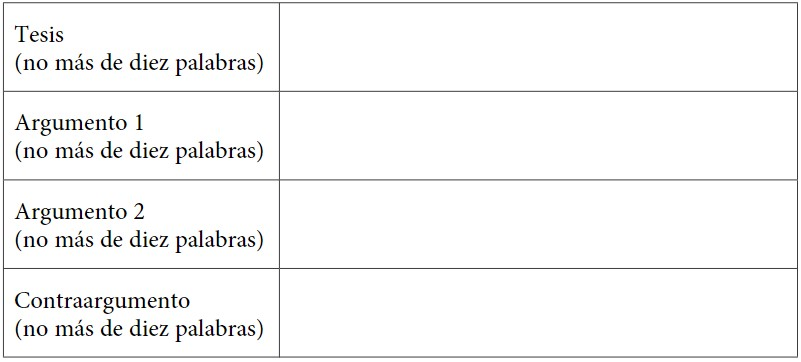
\includegraphics[width=0.7\linewidth]{figures/cuadro_argumentos}
	\caption{Cuadro a completar para realizar un texto argumentativo. }
	\label{fig:cuadroargumentos}
\end{figure}

También podemos ver una serie de conectores relacionados con estos textos:
\begin{itemize}
\item Contraste: a pesar de lo dicho, por el contrario, en cambio, sin embargo, a pesar de...
\item Comparación: de modo similar, de igual forma, de manera semejante, igualmente, así también...
\item Conclusión: mejor dicho, en otros términos, para finalizar, se puede concluir, para concluir...
\item Concesión: por supuesto que, asumiendo, ciertamente, evidentemente, como es evidente...
\item Consecuencia: según lo comentado, por este motivo, de aquí que, de acuerdo con...
\end{itemize}

\item Descriptivo: Este tal vez sea el más complicado, porque te pueden preguntar sobre ejemplo que subrayes cuatro adjetivos, numerales o metáforas. 

\item Expositivos: Este diría que es el más fácil, en este texto te piden subrayar cuatro recursos propios, una definición, clasificación o ejemplificación.
\end{itemize}

\pagebreak

\subsection{Reescribir (completar) Texto}
En esta pregunta se tienen que rellenar unas frases cortas. Puede ser que se traten de conceptos gramáticos, normativos, de conexión (conectores) o léxicos. 

A continuación voy a repasar unas cuestiones que pueden ayudar:
\begin{itemize}
	
\item Leísmo: Uso incorrecto de \textit{le(s)} en lugar de \textit{lo} (en función de CD)
\item Laísmo: Uso incorrecto de \textit{la(s)} en lugar de \textit{le(s)} (en función de CI femenino)
\item Loísmo: Uso incorrecto de \textit{lo(s)} en lugar de \textit{le(s)} (en función de CI masculino)
\item Sino/Si no: \textit{Sino} es una conjunción adversativa ('\textit{no lo hizo él, sino ella}') mientras que \textit{si no} es la conjunción condicional \textit{si} y el adverbio de negación \textit{no} ('\textit{Que lo haga él y, si no, ella}')
\item Porque/Porqué: \textit{Porque} sería el que utilizamos para explicar o responder, mientras que el \textit{porqué} es el de \textit{'explícame el porqué'}. 
\item Sí/Si: 
\item Voy/Vengo:
\item Tí/Ti:
\item Aun/Aún: 
\item Había/Habían:
\item Con que/Conque: 
\item Mío/De mí: 
\item Desde/Des de:
\item Siquiera/Si quiera:
\item Donde/Dónde: 


\subsection{Otros términos}
\begin{itemize}

\item Complemento predicativo: complemento que funciona como CCM pero siendo un adjetivo. 
\item V. Transitivo: Verbo que requiere un CD. Piensa en el verbo \textit{haber}, por ejemplo. 

\end{itemize}


	
\end{itemize}
	
\end{document}